\documentclass{eeict}
\inputencoding{utf8}
\usepackage[bf]{caption2}
\usepackage{amssymb}
\usepackage{amsmath}
\usepackage{dsfont}
\usepackage{graphicx}
\usepackage{multirow}


\newtheorem{example}{Example}[section]
%--------------------------------------------------------------------------------

\title{A decision procedure for the WS$k$S logic}
\author{Tomáš Fiedor}
\programme{Master Degree Programme 2, FIT BUT}
\emails{xfiedo01@stud.fit.vutbr.cz}

\supervisor{Ondřej Lengál}
\emailv{ilengal@fit.vutbr.cz}

\abstract{Various types of logics are often used as a means for a formal
specification of systems. The weak monadic second-order logic with $k$
successors (WS$k$S) is one of these logics with quite high expressivity, yet
still decidable. Although the complexity of checking satisfiability of
a WS$k$S formula is not even in the ELEMENTARY class, there are some approaches
to this problem that perform well in practice. The currently existing
implementations of a WS$k$S decision procedures are based on the use of
deterministic tree automata. The aim of this work is to exploit the recently
developed techniques for efficient manipulation of non-deterministic tree
automata and implement an efficient WS$k$S decision procedure based on those.}
\keywords{formal verification, tree automata, WS$k$S, decision procedures}

\begin{document}

\maketitle

%-------------------------------------------------------------------------------
\selectlanguage{english}
\section{Introduction}

In formal verification, logics are often used for a specification of the
verified systems in a very natural and intuitive way. The \emph{weak monadic
second-order logic of $k$ successors} (WS$k$S) \cite{wsks} is a fragment of the
second order monadic logic that allows to quantify over finite set variables
where every element from the universe of discourse has $k$ successors. This way
various $k$-ary tree structures, e.g.
heaps or binary trees, and linear structures, e.g. linked lists, can be expressed.

There has been established a
one-to-one correspondence between WS$k$S formulae and tree automata. Based
on this there has already been several attempts to implement a~decision
procedure for WS$k$S using deterministic tree automata \cite{mona}. However,
with the recent development in algorithms for manipulation of
non-deterministic tree automata, the aim of this work is to exploit these ideas
in an implementation of a WS$k$S decision procedure based on non-deterministic
tree automata.

\section{WS$k$S syntax}

A WS$k$S \emph{term} is either the empty constant $\epsilon$, a first-order
variable symbol written in lower-case letters (e.g. $x$, $y$, \ldots) or an
unary symbol from $\{1,\ldots,k\}$ written in postfix notation. For example
$x1123$ or $\epsilon2111$ are terms. An \emph{atomic formula}, for some
second-order variables $X$ and $Y$, is either the subset predicate $X
\subseteq Y$, the singleton predicate $Sing(X)$, the successor predicate $X =
Yi$, for some $1 \leq i \leq k$, or predicate $X
= \epsilon$ denoting that $X$ is a singleton set $\{\epsilon\}$.
A WS$k$S \emph{formula} is then built out of these atomic formulae using only the
logical connectives $\wedge, \vee, \neg$ and the existential quantifier $\exists
X$ for quantification over second-order variables.

\begin{example} The following example WS$k$S formula $\varphi$ denotes that there
exists a singleton set which is not a subset of the set $X$.
\begin{equation}
 \psi \overset{\mathit{def}}{=} \neg\exists P: Sing(P) \wedge P
 \not\subseteq X
 \label{varphi}
\end{equation}
\end{example}

\section{Deciding WS$k$S}

Many decision procedures for a wide range of logics are based on the use of some
kind of finite-state automata. WS$k$S is no exception and its currently most
often used decision procedure is based on constructing a $k$-ary tree automaton
and examining its language.

\subsection{Deciding WS$k$S using deterministic automata}

One of the tools for deciding WS$k$S, MONA \cite{mona}, constructs a
deterministic tree automaton $\mathcal{A}_\varphi$ for the given formula
$\varphi$ recursively on the structure of the formula. As a base, each atomic
subformula is transformed to a corresponding automaton.
Further it constructs for connectives $\phi \vee
\psi$, $\phi \wedge \psi$, $\neg \phi$ and $\exists X. \phi$, union of
$\mathcal{A}_\phi$ and $\mathcal{A}_\psi$, intersection of $\mathcal{A}_\phi$
and $\mathcal{A}_\psi$, complement of $\mathcal{A}_\phi$ and projection on the
track of $X$ of $\mathcal{A}_\phi$ respectively, such an automaton then
represents all models of formula $\varphi$.


\begin{figure}
 \begin{center}
  \scalebox{0.55}{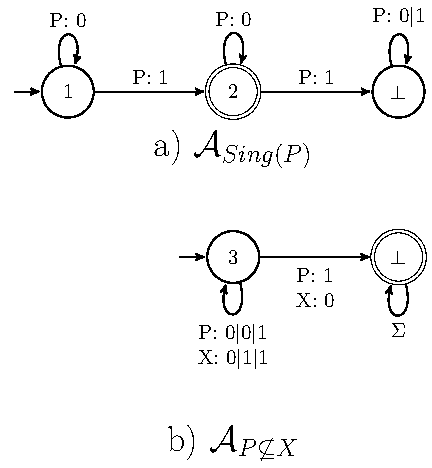
\includegraphics{formula-singleton-and-subset.pdf}}
  \scalebox{0.55}{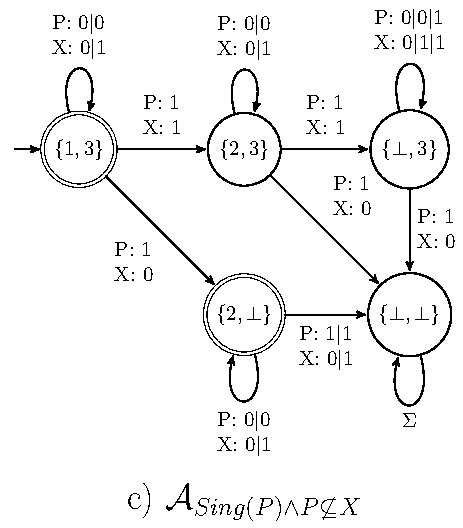
\includegraphics{formula-automaton-product.pdf}}
  \scalebox{0.55}{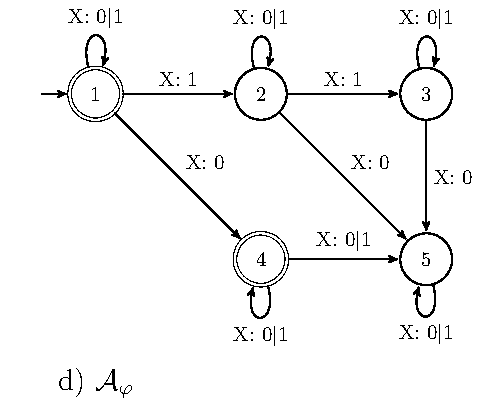
\includegraphics{formula-automaton.pdf}}
 \end{center}
 \caption{Finite automata corresponding to the subformulae of the formula
 $\varphi \overset{\mathit{def}}{=} \exists P:
 Sing(P) \wedge P \not\subseteq X$}\label{example}
\end{figure}

\subsection{Deciding WS$k$S using non-deterministic automata}

Although this approach yields good results in many practical examples, every
time non-determinism is introduced the automaton is determinised and the
information about the original states is forgotten. Therefore such an approach
has issues with extensive use of automaton complementation and since currently
there is no known tree automaton complementation technique better than bottom-up determinization of automaton with complementation of the
set of final states, heavy optimizations and heuristics had to be used in MONA
to achieve good results.

We propose that it is not necessary to construct the automaton representing all
models of $\varphi$. Instead construction of the automaton and the search for an
accepting or a non-accepting state can be done \emph{on-the-fly} and we can further exploit
recent development in algorithms for manipulating non-deterministic
tree automata.
Given a WS$k$S formula $\varphi$ we transform it to the formula in the \emph{existentially-quantified prenex normal form} $\psi \overset{\mathit{def}}{=}
\exists\mathcal{X}_{m+1}\neg\exists\mathcal{X}_m\ldots\neg\exists\mathcal{X}_2\neg\exists\mathcal{X}_1.\pi(\mathds{X})$,
where $\mathcal{X}_i$ denotes a set of second order variables.
We then create a hierarchical family of formulae $\Phi =
\{\varphi_0,\ldots,\varphi_m\}$ where $\varphi_0 \overset{\mathit{def}}{=} \pi$ and for all $0 \leq i \leq
m-1$ it holds that $\varphi_{i+1} \overset{\mathit{def}}{=}
\neg\exists\mathcal{X}_{i+1}.\,\varphi_i$.

Further, using the operations of complementation $\gamma$ and projection
$\omega_{\mathcal{X}}$ over the set of variables $\mathcal{X}$, we define the
family of automata $\mathds{A} = \{\mathcal{A}_0,\ldots,\mathcal{A}_m\}$ as follows:
\begin{eqnarray}
 \mathcal{A}_0 & = & \mathcal{A}_\pi\\
 \mathcal{A}_{i+1} & = & \gamma(\omega_{\mathcal{X}_{i+1}} (\mathcal{A}_i))
\end{eqnarray}
such that there is a correspondence between $\mathcal{A}_i$ and $\varphi_i$ for
all $0 \leq i \leq m$.

The Language of the automaton $\mathcal{A}_\psi$ is further tested for
universality.
The classical naive approach performs determinization using subset construction
to obtain a deterministic automaton, which is further complemented by
swapping final and non-final states and finally checked whether it contains
reachable final state. In our approach we wish to exploit the ideas from the
Antichains algorithm \cite{anti} and check universality of $\mathcal{A}_\psi$
without explicitly constructing it, but rather using a search of the state space
over powers of the state set of $\mathcal{A}_0$. To illustrate this on an
example, consider the example formula $\psi \overset{\mathit{def}}{=}
\neg\exists P:
 Sing(P) \wedge\neg P \subseteq X$ and the automaton
$\mathcal{A}_\varphi$ from Figure 1 corresponding to the formula $\varphi
\overset{\mathit{def}}{=} \exists P:
 Sing(P) \wedge\neg P \subseteq X$, i.e. $\psi \overset{\mathit{def}}{=} \neg
 \phi$. We can search for a non-accepting state of $\mathcal{A}_\psi$ by
 searching for a reachable set of states of $\mathcal{A}_\varphi$ that does not
 contain a final state. Further, by using the antichains principle, if we
 encounter a set of states $P$ and later a set of states $R$, s.t. $P \subseteq
 R$, we do not need to explore $R$ as $P$ is smaller and therefore has a bigger
 chance of reaching a non-accepting set of states.

\begin{figure}
 \begin{center}
  \scalebox{0.5}{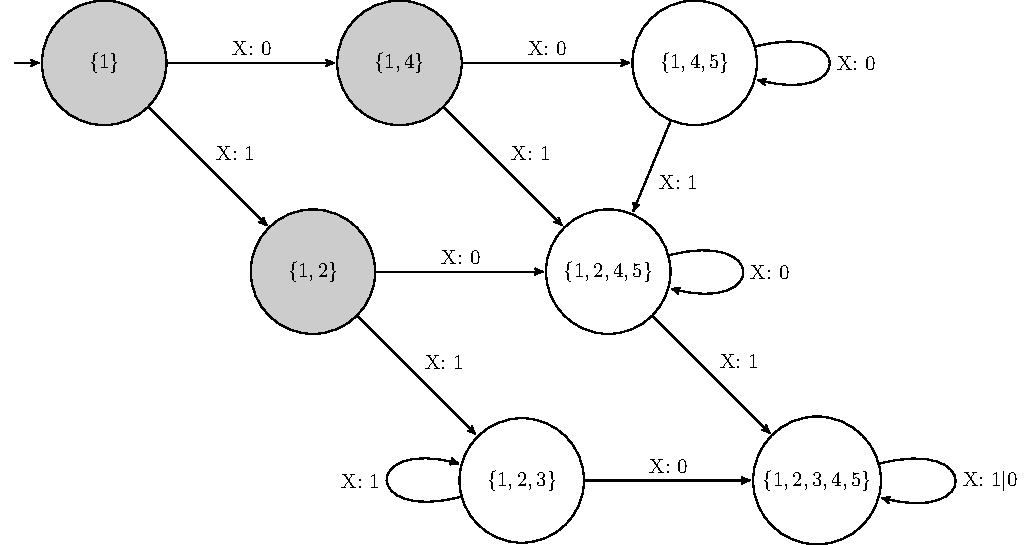
\includegraphics{antichain-meets-projection.pdf}}
 \end{center}
 \caption{Comparison of the antichain-based (grey nodes) and the classical
 approach to universality checking of the automaton $\mathcal{A}_\psi$
 corresponding to the formula $\psi \overset{\mathit{def}}{=} \neg\exists P:
 Sing(P) \wedge\neg P \subseteq X$}\label{compare}
\end{figure}

\section{Conclusion}

We proposed a new decision procedure of WS$k$S logic that uses non-deterministic
automata instead of deterministic ones used, e.g. in tool
MONA \cite{mona}. This different approach makes use of recent developments in
the field of non-deterministic automata algorithms such as universality
checking or language inclusion checking, allowing us to search for a rejecting or accepting
states on-the-fly without constructing the automaton corresponding to the given
formula at all, possibly yielding a~faster decision procedure for some class of formulae.

%------------
% Citace
%------------
\begin{thebibliography}{9}
%  \bibitem{anti}Abdulla, Parosh Aziz, Hol\'{i}k, Luk\'{a}\v{s}, Chen, Yu-Fang,
%  Mayr, Richard, Vojnar, Tom\'{a}\v{s}.: When simulation meets antichains (on
%  checking language inclusion on nondeterministic finite (tree) automata). In
%  \emph{Tools and Algorithms for Construction and Analysis of Systems}, LNCS
%  6015, pages 158-174, Springer Verlag, 2010.
\bibitem{anti}Abdulla, Parosh Aziz et al.: When simulation meets
antichains (on checking language inclusion on nondeterministic finite (tree) automata). In
  \emph{Tools and Algorithms for Construction and Analysis of Systems}, LNCS
  6015, pages 158--174, Springer Verlag, 2010.
  \bibitem{mona}MONA:
  Web pages of MONA.
  [online] Available on:
  http://www.brics.dk/mona/.
  \bibitem{tata}Comon, H. et al.: Tree automata techniques and applications.
  2007, release October 12th, 2007.
  \bibitem{wsks}Büchi, J. R.: Weak second-order arithmetic and finite automata.
  \emph{Mathematical Logic Quarterly}, 6(1--6):66--92, 1960.
\end{thebibliography}

\end{document}
